\chapter{Konzept und Entwurf}

Wie üblich bei einem Projekt startet man mit Mockups der Anwendung, damit der Kunde eine genauere Vorstellung seiner Ideen bekommt. 

Wir haben uns ziemlich stark an unsere Mockups gehalten und im Folgenden sieht man jedes Mockup gepaart mit dem dazugehörigen Screenshot aus der fertigen App.

Wenn man die App öffnet befindet man sich als erstes auf der Startseite.\\

\begin{figure}[h]
    \centering
    \begin{minipage}{0.45\textwidth}
        \centering
        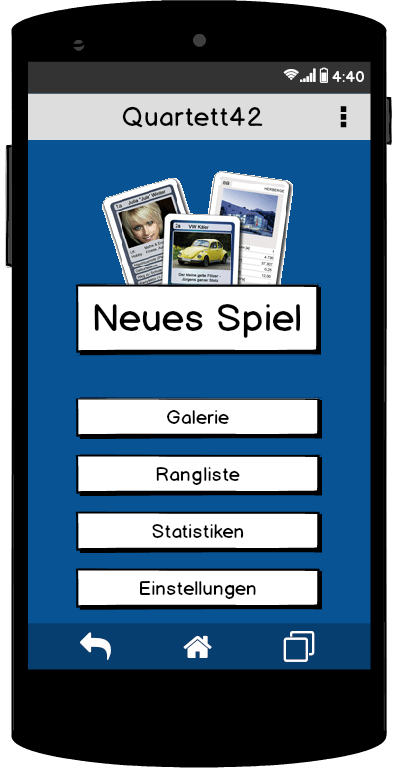
\includegraphics[width=0.75\textwidth]{img/mockups/main_screen.png}
        \caption{first figure}
    \end{minipage}
    \begin{minipage}{0.45\textwidth}
        \centering
        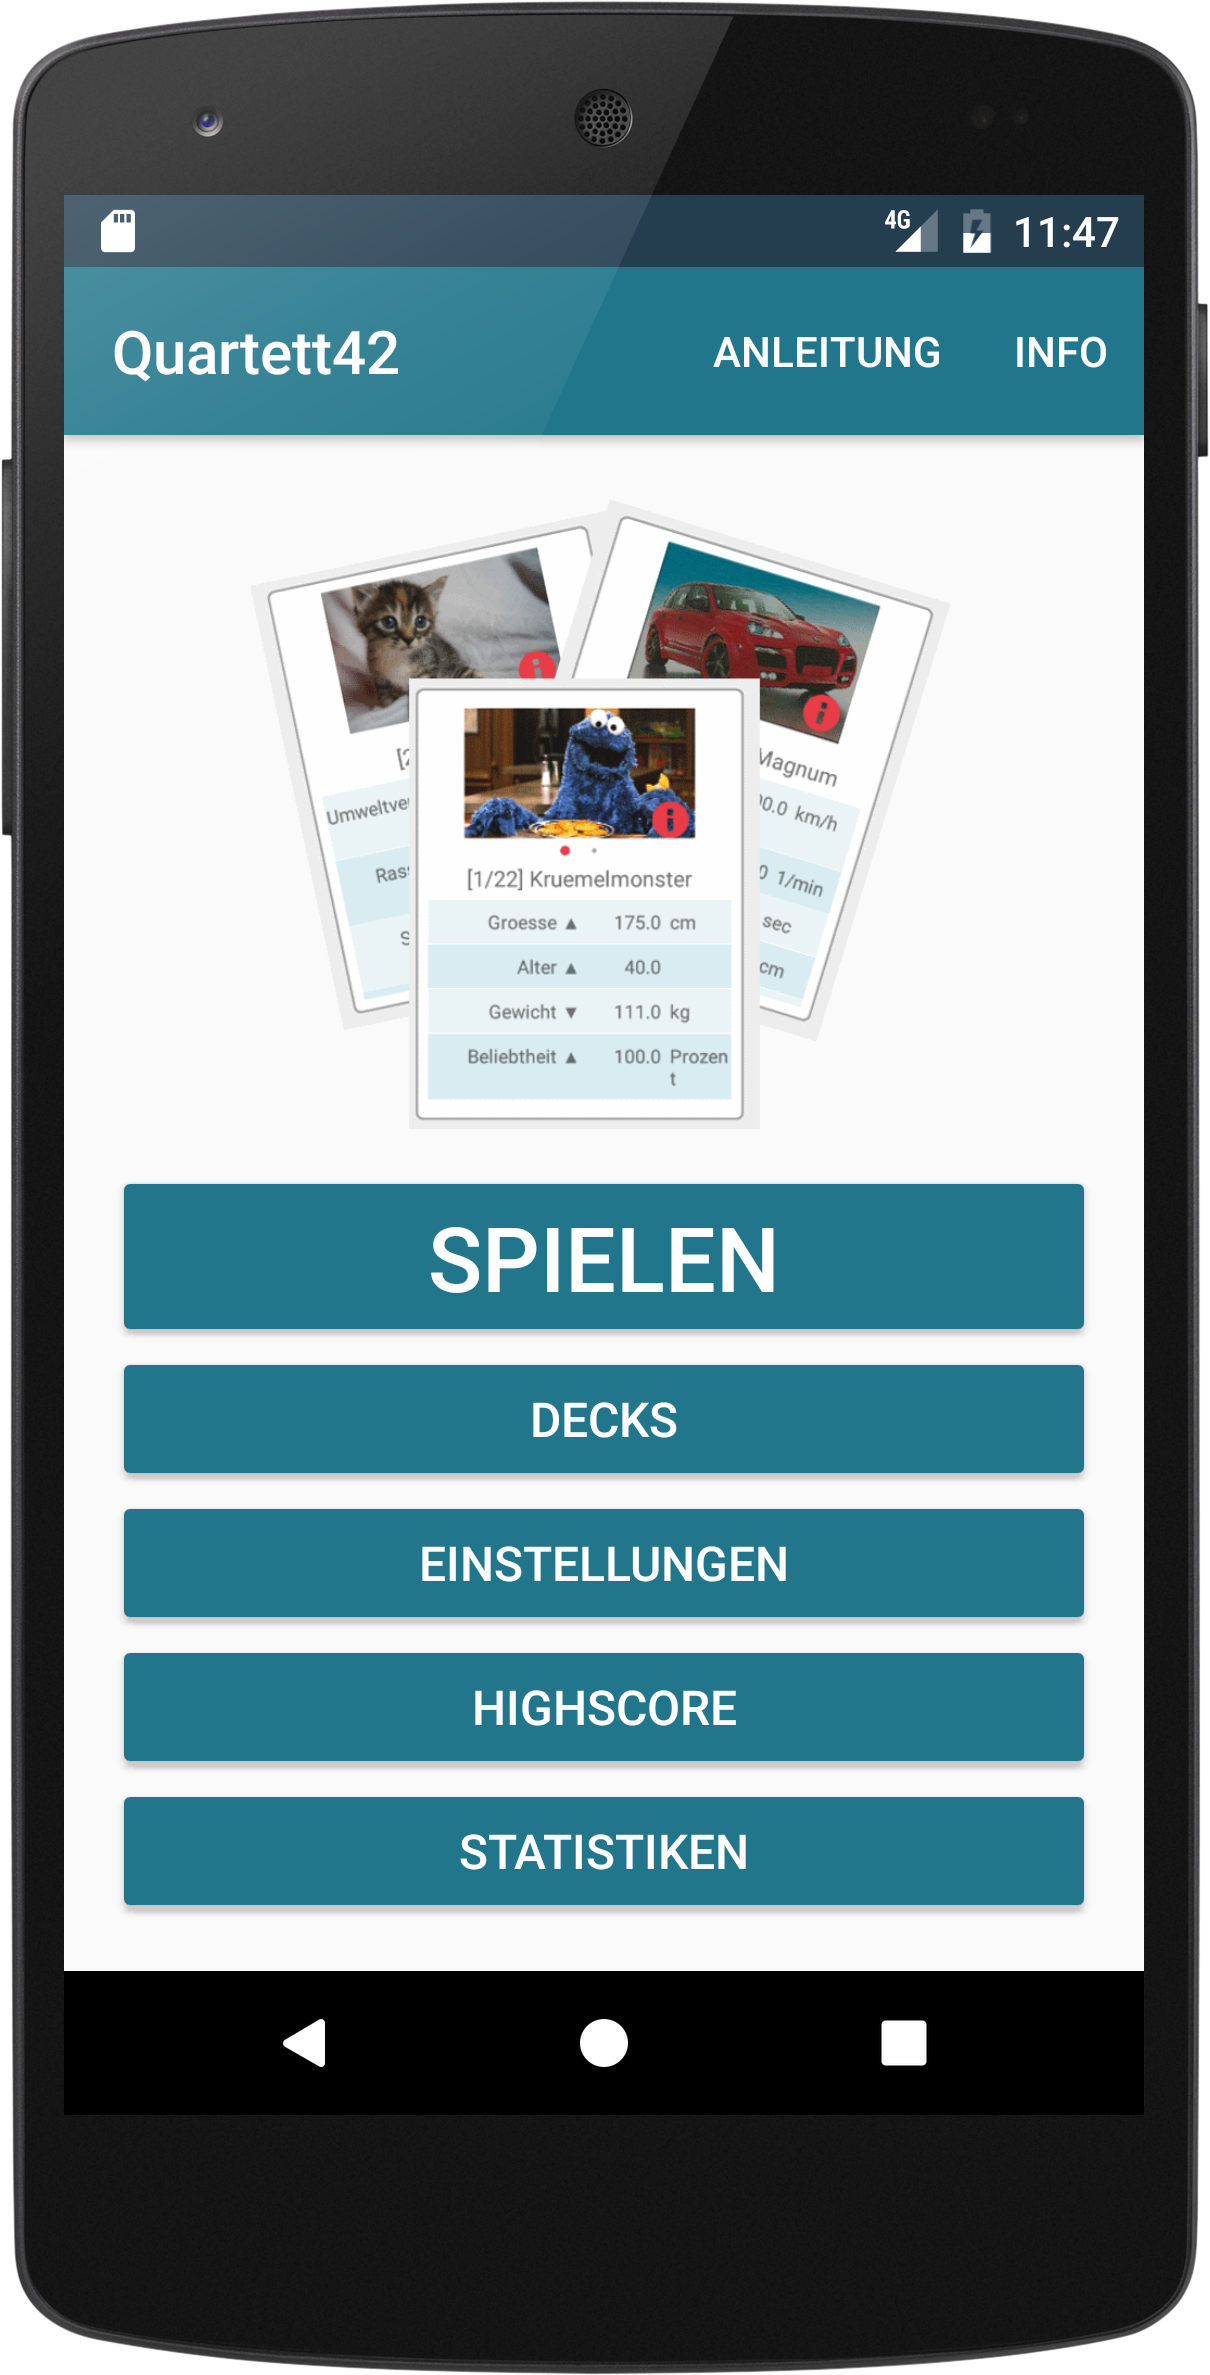
\includegraphics[width=0.75\textwidth]{img/screenshots/device_main_screen.png}
        \caption{second figure}
    \end{minipage}
\end{figure}

Als nächstes manövriert man zu einem neuen Spiel. Hier haben wir, anders als in dem Mockup, die Einstellungen nur angezeigt, aber man kann sie natürlch noch ändern bevor man das Spiel startet. Ein Deck muss aber jedes mal gewählt werden. \\

\begin{figure}[h]
    \centering
    \begin{minipage}{0.45\textwidth}
        \centering
        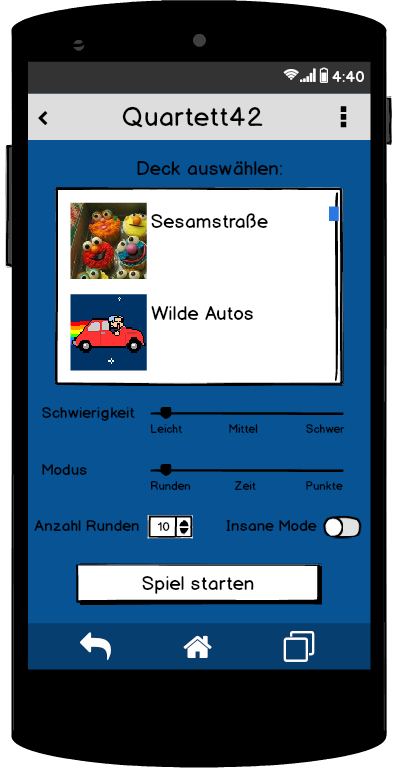
\includegraphics[width=0.4\textwidth]{img/mockups/neues_spiel.png}
        \caption{first figure}
    \end{minipage}\hfill
    \begin{minipage}{0.45\textwidth}
        \centering
        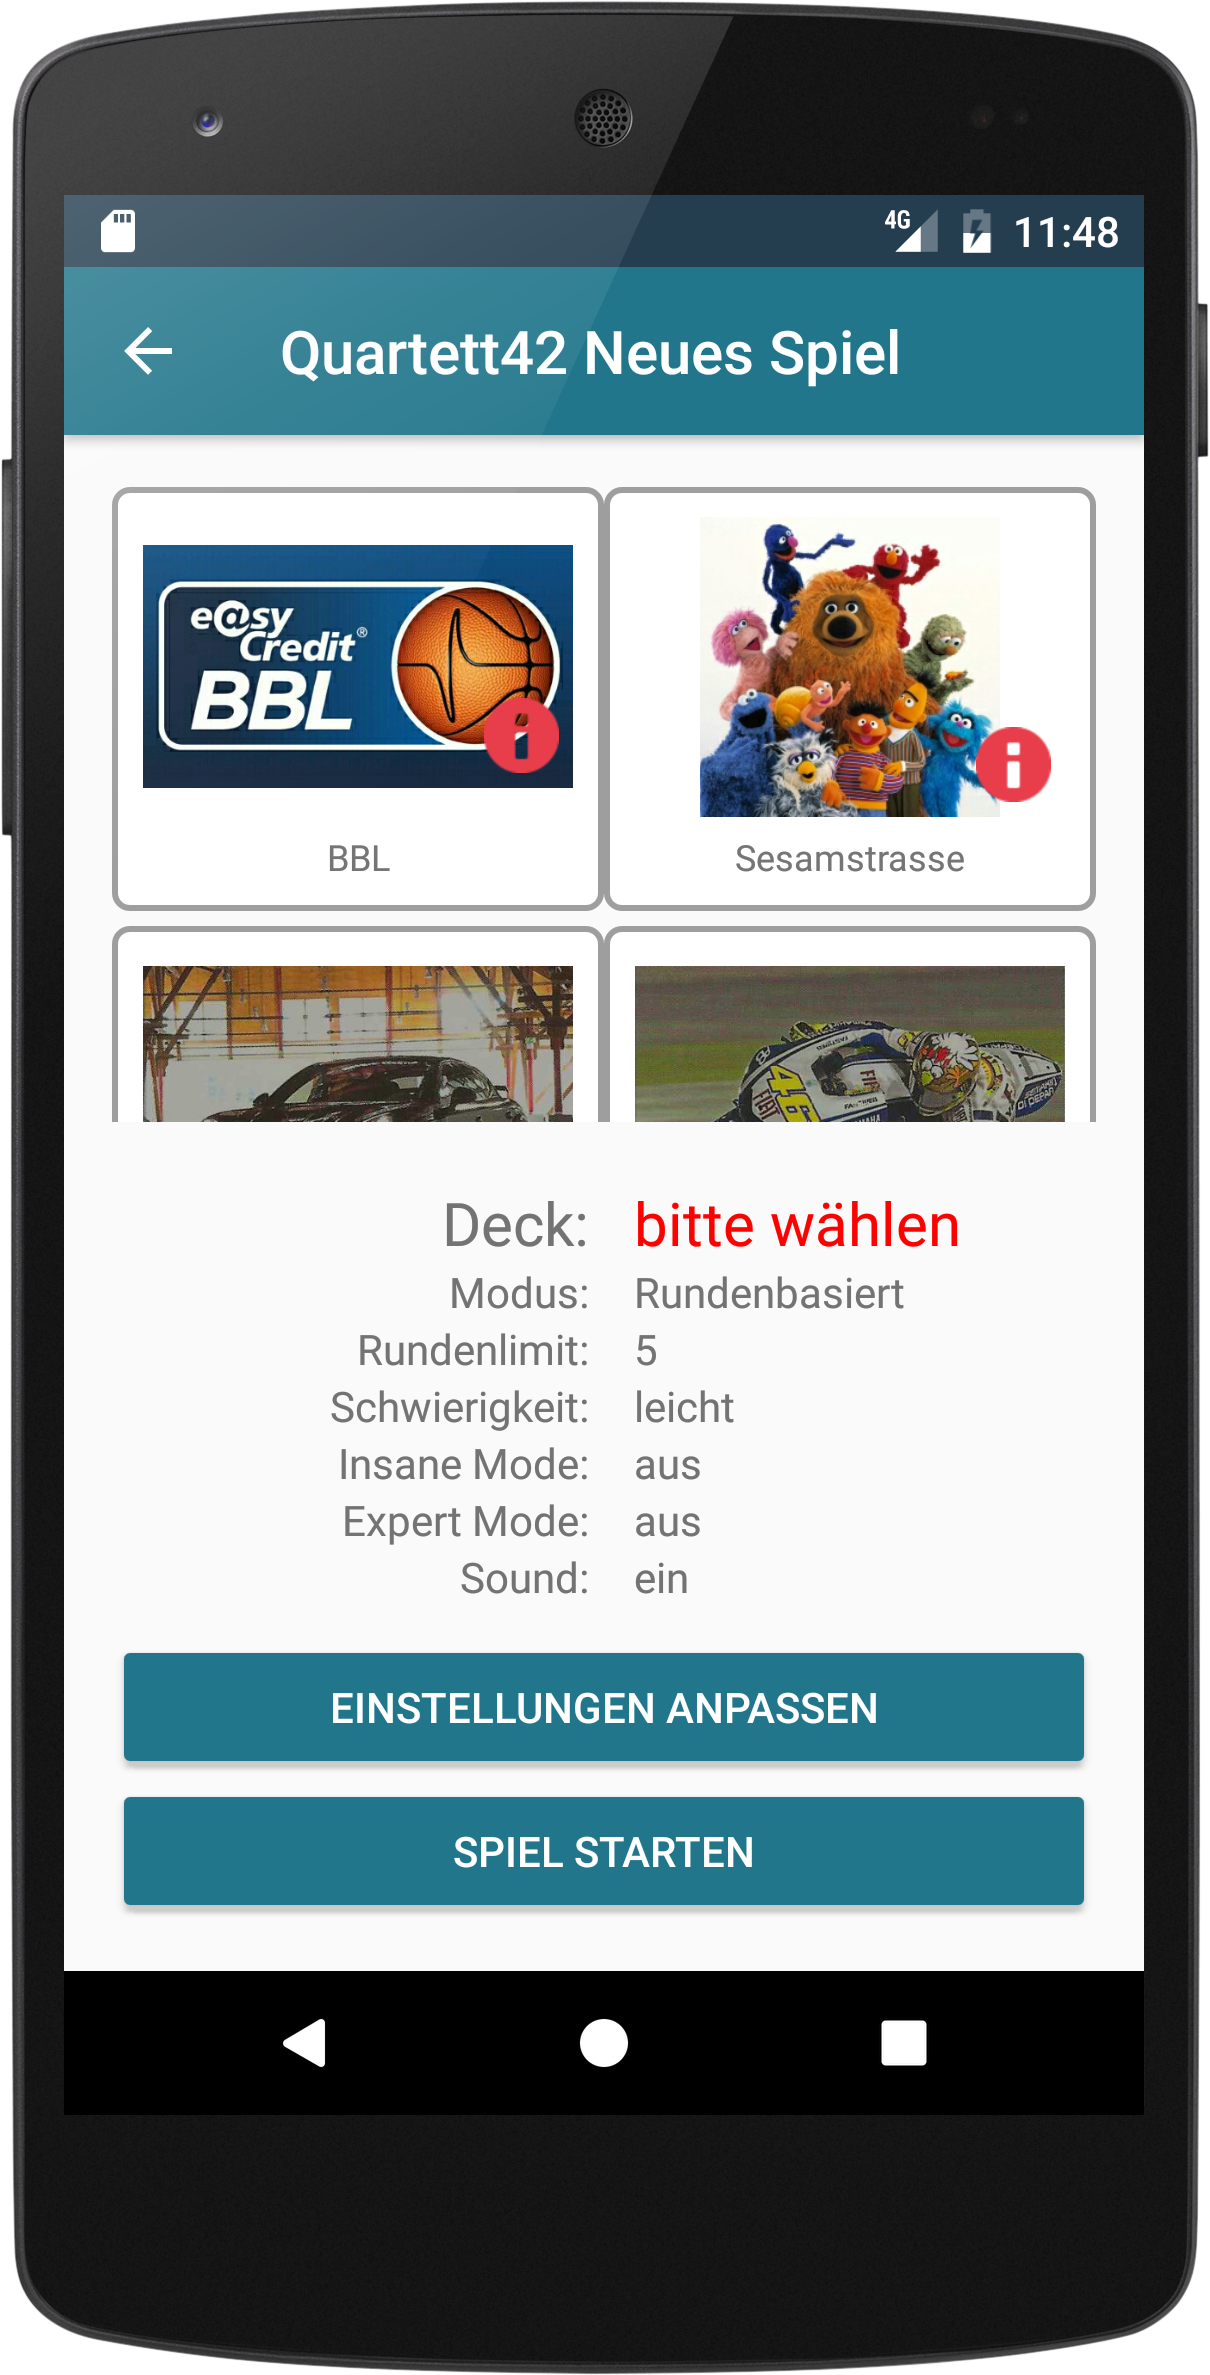
\includegraphics[width=0.4\textwidth]{img/screenshots/device_new_game.png}
        \caption{second figure}
    \end{minipage}
\end{figure}

Will man jetzt doch noch etwas an den Einstellungen ändern, tippt man auf Einstellungen anpassen und kann nun beliebig Anpassungen vornehmen.

\begin{figure}[h]
    \centering
    \begin{minipage}{0.45\textwidth}
        \centering
        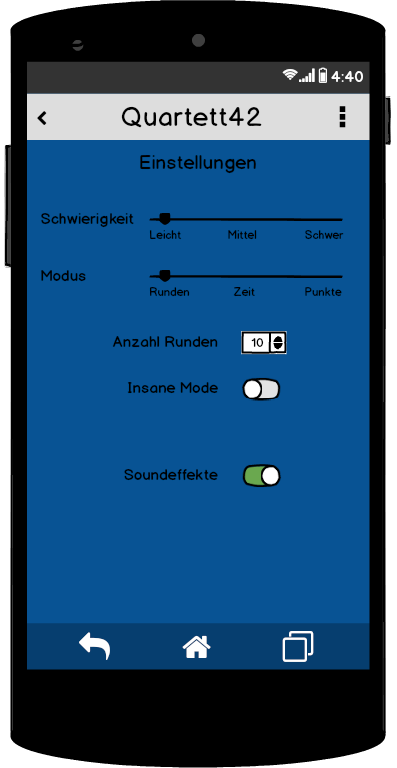
\includegraphics[width=0.4\textwidth]{img/mockups/einstellungen.png}
        \caption{first figure}
    \end{minipage}\hfill
    \begin{minipage}{0.45\textwidth}
        \centering
        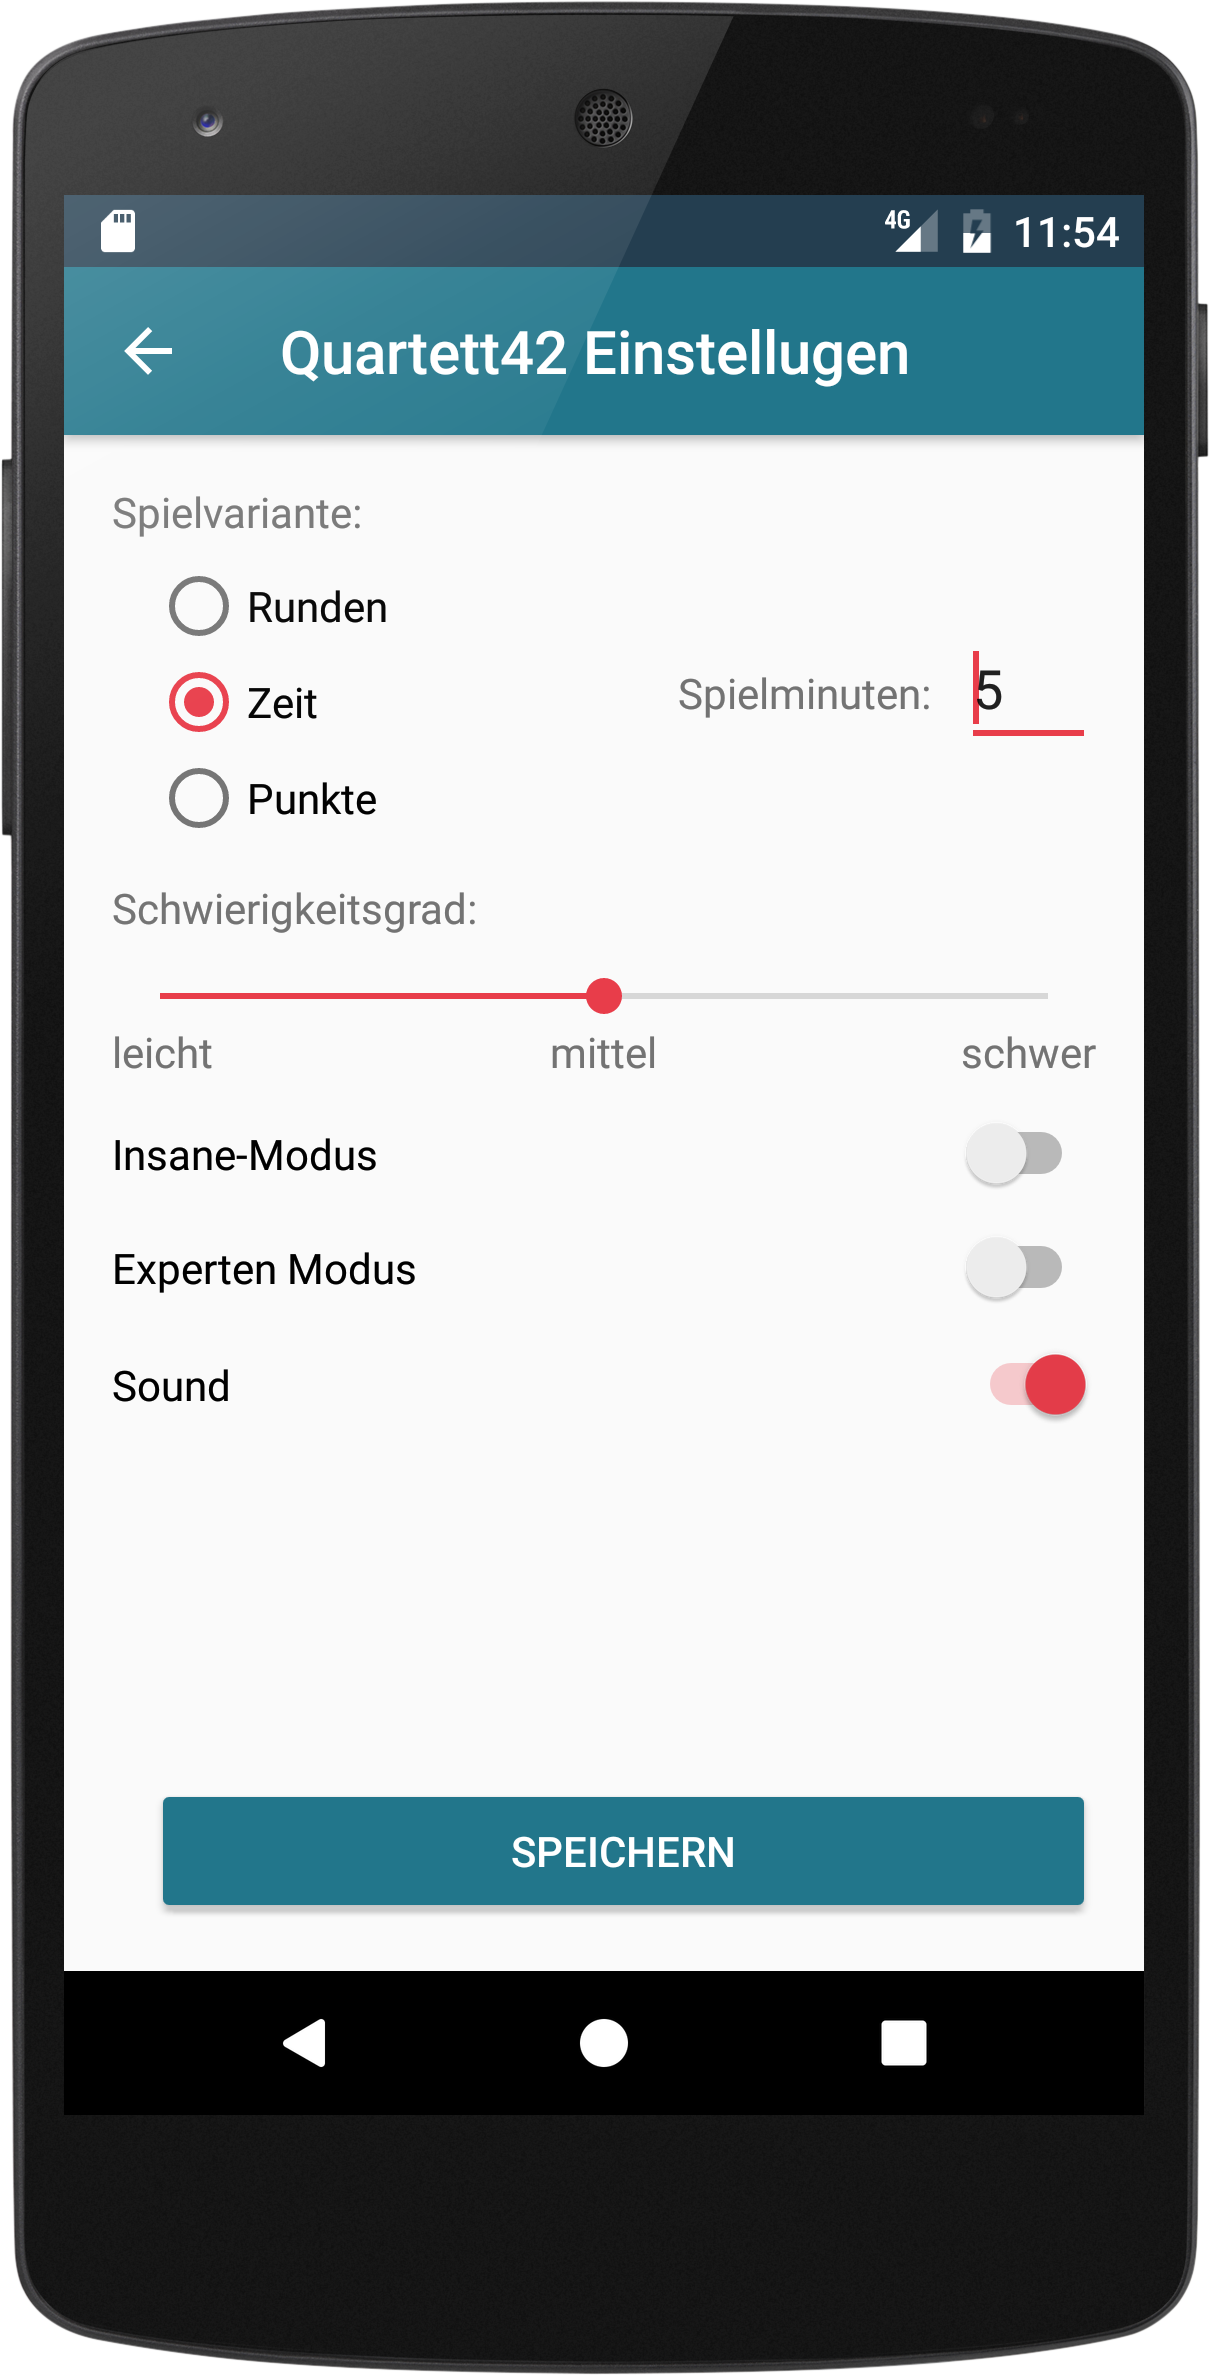
\includegraphics[width=0.4\textwidth]{img/screenshots/device_settings.png}
        \caption{second figure}
    \end{minipage}
\end{figure}
